
\documentclass[tikz]{standalone}
\usepackage{graphicx}
\usepackage{lmodern}
\usepackage{amsmath, amssymb, amsfonts}
\usetikzlibrary{calc}
\newcommand{\R}{\mathcal{R}}

\begin{document}

%n = 5, d = 2 construction proof intuition for abstain
\begin{tikzpicture}
%draw axes
\draw[<->, dashed, opacity = 0.3] (-2, 0) -- (2,0);
\draw[<->, dashed, opacity = 0.3] (0, -2) -- (0,2);

%v_1
\draw[->, thick] (0,0) -- (0,1);
\node at (0.2, 0.8){\footnotesize$v_1$};
%\draw[dashed, opacity = 0.5](-2, 1) -- (2,1);
%\draw[dashed, opacity = 0.5](-2, -1) -- (2,-1);


%v_2
\draw[->, thick] (0,0) -- (1/4,1/4);
\node at (0.3, 0.4){\footnotesize$v_2$};
%\draw[dashed, opacity = 0.5](-3/2, 2) -- (2,-3/2);
%\draw[dashed, opacity = 0.5](-2, 3/2) -- (3/2,-2);


%line for v2 .x = 1
%y = -x - 1/2


%v_3
%\draw[->, thick] (0,0) -- (2/3,1/3);
%\node at (0.5, 0.1){\footnotesize$v_3$};
%\draw[dashed, opacity = 0.5](-1/6,2) -- (11/6,-2);
%\draw[dashed, opacity = 0.5](-11/6, 2) -- (1/6, -2);

%%calculating lines for v3
%%x = -1/2 y + 5/6
%%x = -1/2 y - 5/6


%label nodes of intersection
%\node at (3/2,-1) {\footnotesize$x^{12}_1$};
%\node at (-3/2, 1) {\footnotesize$x^{12}_2$};
%\node at (4/3, -1) {\footnotesize$x^{13}_1$};
%\node at (-4/3, 1) {\footnotesize$x^{13}_3$};

%label feasible regions
%\path[fill = red, opacity= 0.2] (-2, -1) -- (4/3,-1)-- (11/6,-2)-- (-2, -2) -- cycle;
%\node at (-1,-3/2) {$F_1$};
%
%\path[fill = blue, opacity= 0.2] (-2, 1) -- (-3/2,1)-- (3/2,-2)-- (-2, -2) -- cycle;
%\node at (-3/2,1/2) {$F_2$};
%
%\path[fill = yellow, opacity= 0.2] (-2, 1) -- (-4/3,1)-- (1/6,-2)-- (-2, -2) -- cycle;
%\node at (-4/3, -1/2) {$F_3$};

\end{tikzpicture}

%n = 5, d = 2 construction proof intuition for abstain
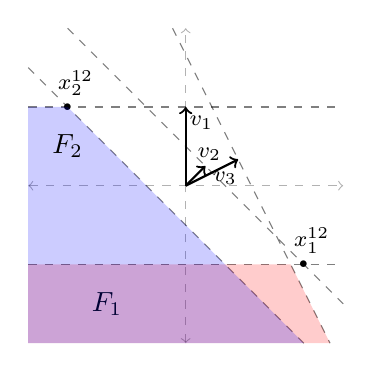
\begin{tikzpicture}
%draw axes
\draw[<->, dashed, opacity = 0.3] (-2, 0) -- (2,0);
\draw[<->, dashed, opacity = 0.3] (0, -2) -- (0,2);

%v_1
\draw[->, thick] (0,0) -- (0,1);
\node at (0.2, 0.8){\footnotesize$v_1$};
\draw[dashed, opacity = 0.5](-2, 1) -- (2,1);
%\path[fill = blue, opacity = 0.2] (-2,1) -- (2,1) -- (2,2) -- (-2,2) -- cycle;
\draw[dashed, opacity = 0.5](-2, -1) -- (2,-1);
%\path[fill = blue, opacity = 0.2] (-2,-1) -- (2,-1) -- (2,-2) -- (-2,-2) -- cycle;

%v_2
\draw[->, thick] (0,0) -- (1/4,1/4);
\node at (0.3, 0.4){\footnotesize$v_2$};
\draw[dashed, opacity = 0.5](-3/2, 2) -- (2,-3/2);
\draw[dashed, opacity = 0.5](-2, 3/2) -- (3/2,-2);


%line for v2 .x = 1
%y = -x - 1/2


%v_3
\draw[->, thick] (0,0) -- (2/3,1/3);
\node at (0.5, 0.1){\footnotesize$v_3$};
\draw[dashed, opacity = 0.5](-1/6,2) -- (11/6,-2);
%\path[fill = yellow, opacity = 0.2] (-1/6,2) -- (2,2) -- (2,-2) -- (11/6,-2) -- cycle;
%\draw[dashed, opacity = 0.5](-11/6, 2) -- (1/6, -2);
%\path[fill = yellow, opacity = 0.2] (-2,2) -- (-11/6,2) -- (1/6,-2) -- (-2,-2) -- cycle;

%calculating lines for v3
%x = -1/2 y + 5/6
%x = -1/2 y - 5/6


%label nodes of intersection
\node[label={[xshift=0.1cm, yshift=-0.15cm]{\footnotesize$x^{12}_1$}}] at (3/2,-1) {\Huge$.$};
\node[label={[xshift=0.1cm, yshift=-0.15cm]{\footnotesize$x^{12}_2$}}] at (-3/2,1) {\Huge$.$};
%\node at (4/3, -1) {\footnotesize$x^{13}_1$};
%\node at (-4/3, 1) {\footnotesize$x^{13}_3$};

%label feasible regions
\path[fill = red, opacity= 0.2] (-2, -1) -- (4/3,-1)-- (11/6,-2)-- (-2, -2) -- cycle;
\node at (-1,-3/2) {$F_1$};

\path[fill = blue, opacity= 0.2] (-2, 1) -- (-3/2,1)-- (3/2,-2)-- (-2, -2) -- cycle;
\node at (-3/2,1/2) {$F_2$};

%\path[fill = yellow, opacity= 0.2] (-2, 1) -- (-4/3,1)-- (1/6,-2)-- (-2, -2) -- cycle;
%\node at (-4/3, -1/2) {$F_3$};

\end{tikzpicture}

 


\end{document}
%%% Local Variables:
%%% mode: latex
%%% TeX-master: t
%%% End:
